\def\layersep{5.3cm}
\begin{figure}[H]
    \centering
    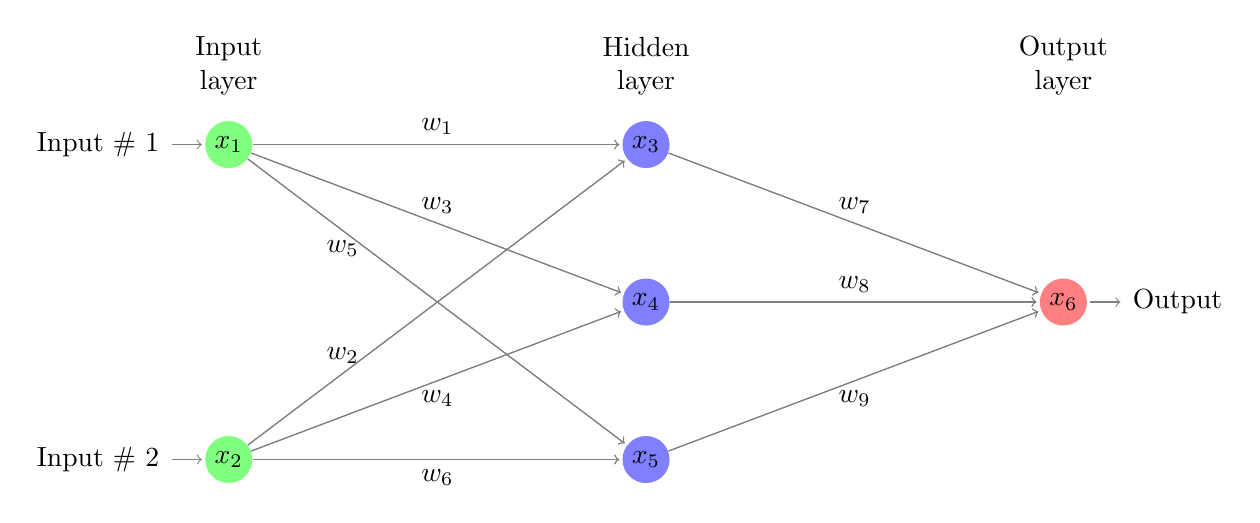
\begin{tikzpicture}[shorten >=1pt,->,draw=black!50, node distance=\layersep]
      \tikzstyle{every pin edge}=[<-,shorten <=1pt]
      \tikzstyle{neuron}=[circle,fill=black!25,minimum size=17pt,inner sep=0pt]
      \tikzstyle{input neuron}=[neuron, fill=green!50];
      \tikzstyle{output neuron}=[neuron, fill=red!50];
      \tikzstyle{hidden neuron}=[neuron, fill=blue!50];
      \tikzstyle{annot} = [text width=4em, text centered]
  
      % Draw the input layer nodes
      \foreach \name / \y in {1,...,2}
      % This is the same as writing \foreach \name / \y in {1/1,2/2,3/3,4/4}
          \node[input neuron, pin=left:Input \# \y] (I-\name) at (0,4*-\y + 3) {\(x_{\y}\)};
  
      % Draw the hidden layer nodes
      \foreach \name / \y in {3,...,5}
          \path[yshift=1cm]
              node[hidden neuron] (H-\name) at (\layersep,2*-\y + 4) {\(x_{\y}\)};
  
      % Draw the output layer node
      \node[output neuron,pin={[pin edge={->}]right:Output}, right of=H-4] (0) {\(x_6\)};
  
      % Connect every node in the input layer with every node in the
      % hidden layer.
      \foreach \source in {1,...,2}
          \foreach \dest in {3,...,5}
              \path (I-\source) edge (H-\dest);
  
      % Connect every node in the hidden layer with the output layer
      \foreach \source in {3,...,5}
          \path (H-\source) edge (0);
  
      % Annotate the layers
      \node[annot,above of=H-3, node distance=1cm] (hl) {Hidden layer};
      \node[annot,left of=hl] {Input layer};
      \node[annot,right of=hl] {Output layer};
      \draw (I-1) -- (H-3) node[midway, above]{\(w_1\)};
      \draw (I-2) -- (H-3) node[near start, above]{\(w_2\)};
      \draw (I-1) -- (H-4) node[midway, above]{\(w_3\)};
      \draw (I-2) -- (H-4) node[midway, below]{\(w_4\)};
      \draw (I-1) -- (H-5) node[near start, below]{\(w_5\)};
      \draw (I-2) -- (H-5) node[midway, below]{\(w_6\)};
      \draw (H-3) -- (0) node[midway, above]{\(w_7\)};
      \draw (H-4) -- (0) node[midway, above]{\(w_8\)};
      \draw (H-5) -- (0) node[midway, below]{\(w_9\)};
  \end{tikzpicture}


    \caption{Neural network.}\label{fig:neural_net}
\end{figure}